\chapter{Dynamique de Friedmann et équation d’état}

\lectureoverview{L’expansion homogène doit être distinguée de la physique locale des systèmes liés, et la géométrie intrinsèque de la forme d’un plongement. Une fois ces distinctions bien établies, le principe cosmologique ramène la métrique de l’espace-temps à un seul facteur d’échelle \(a(t)\) et un seul paramètre de courbure \(k\). La composante temporelle de l’équation d’Einstein devient alors l’équation de Friedmann pour l’énergie. Pour la résoudre, il nous faut encore la relation entre la pression et la densité d’énergie caractéristique de la matière. La thermodynamique adiabatique et l’équation d’état \(P=w\rho\) donnent \(\rho\propto a^{-3(1+w)}\), unifiant la matière, le rayonnement et l’énergie du vide dans un cadre unique.}

\section{Questions qui précisent le tableau physique}

\subsection{L’espace pourrait-il se répéter avant l’horizon ?}

Un univers plat fini peut être représenté par une cellule périodique. Si cette cellule était plus petite que la région observable, la lumière pourrait la traverser et le ciel présenterait des images répétées des mêmes structures. Détecter ces répétitions est plus difficile que de simplement reconnaître une galaxie familière : les images nous parviennent de directions et d’époques différentes et sont modifiées par l’évolution cosmique. La topologie périodique a néanmoins des conséquences observables.

\begin{classroomqa}
\audiencequestion{L’Univers entier pourrait-il être plus petit que l’Univers observable ?}
\lecturerresponse{Un tore à identifications périodiques est la proposition naturelle. Nous observerions alors des copies répétées d’une même région physique, comme si nous nous voyions par une porte dérobée. Les recherches de la périodicité cosmique correspondante n’ont pas fourni d’éléments en sa faveur, mais elles imposent des contraintes aux petites cellules fondamentales. Cette possibilité est géométriquement cohérente, mais ces observations ne favorisent pas un univers plus petit que la région déjà observée. \lecturetimestamp{00:01:17--00:02:33}}
\end{classroomqa}

\subsection{L’expansion n’écarte pas les systèmes liés}

L’expansion cosmique décrit le mouvement à grande échelle de la matière libre dans la géométrie cosmologique moyenne. Elle n’impose pas que toute longueur propre augmente. Les forces électromagnétiques lient les atomes, la gravitation lie les systèmes planétaires et les forces moléculaires ordinaires lient les objets solides. À ces échelles, ces interactions sont immensément plus fortes que la correction cosmologique.

\begin{classroomqa}
\audiencequestion{L’énergie noire provoque-t-elle l’expansion, et pourquoi les atomes ou les orbites planétaires ne s’étendent-ils pas avec l’espace ?}
\lecturerresponse{L’expansion de l’Univers était connue avant la découverte de l’énergie noire. L’énergie noire modifie l’expansion en l’accélérant ; elle n’en est ni la définition ni la cause originelle. Un système lié ne suit pas le flot de Hubble, car ses forces locales dominent. Un fond accéléré peut induire une perturbation infime d’un atome ou d’une orbite, mais les forces de liaison ordinaires rétablissent un état d’équilibre presque inchangé, au lieu de laisser le système se disloquer. \lecturetimestamp{00:02:36--00:06:50}}
\end{classroomqa}

\subsection{L’énergie dans une géométrie dépendant du temps}

L’objection qui reste ne porte pas sur les forces, mais sur le bilan énergétique. Si une orbite liée s’oppose continuellement à une faible perturbation cosmologique, d’où vient l’énergie nécessaire ? Cette question transpose à un espace-temps dépourvu de symétrie globale par translation temporelle une loi de conservation issue d’un fond statique.

\begin{classroomqa}
\audiencequestion{D’où vient l’énergie lorsque les forces de liaison locales s’opposent à l’expansion ?}
\lecturerresponse{Dans un monde statique, la conservation de l’énergie découle de l’invariance par translation temporelle : le fond et ses lois sont identiques lorsque l’on décale une expérience dans le temps. Un espace-temps en expansion n’est pas invariant par translation temporelle en ce sens global ; il n’est donc pas nécessaire qu’il existe une énergie totale unique conservée pour l’ensemble de l’Univers. La conservation locale du tenseur énergie-impulsion reste valable et apparaîtra plus loin sous la forme de l’équation de continuité. Ce qui échoue, c’est l’affirmation naïve selon laquelle une énergie cosmique définie globalement doit rester constante tandis que la géométrie évolue. \lecturetimestamp{00:06:52--00:09:24}}
\end{classroomqa}

\subsection{L’homogénéité est une affirmation à grande échelle}

Le principe cosmologique dépend de l’échelle considérée. L’air d’une pièce fermée peut être presque uniforme à l’échelle de la pièce, mais il est granulaire à l’échelle moléculaire. De même, l’Univers contient des planètes, des galaxies, des amas et des fluctuations de densité. L’homogénéité et l’isotropie décrivent son comportement moyen sur des distances assez grandes pour que ces structures ne privilégient plus ni position ni direction.

\begin{classroomqa}
\audiencequestion{Les structures liées à petite échelle contredisent-elles l’homogénéité et l’isotropie ?}
\lecturerresponse{Non. L’homogénéité exacte échoue à petite échelle, tout comme celle de l’air lorsqu’on résout les molécules individuellement. À des échelles de plusieurs centaines de millions d’années-lumière et au-delà, la distribution observée est approximativement uniforme et indépendante de la direction. Au-delà de la région observable, l’homogénéité reste une hypothèse dont il faut tester les conséquences, et non un fait établi. \lecturetimestamp{00:09:27--00:10:55}}
\end{classroomqa}

\section{L’homogénéité et l’isotropie comme propriétés métriques}

L’homogénéité et l’isotropie sont d’abord des propriétés géométriques, avant de devenir des propriétés dynamiques. L’équation d’Einstein nous indiquera comment la géométrie évolue dans le temps. Il faut d’abord préciser quelles géométries spatiales sont possibles à un instant donné.

\begin{classroomqa}
\audiencequestion{Que signifient mathématiquement l’homogénéité et l’isotropie ?}
\lecturerresponse{Décrivons l’espace à l’aide d’une métrique et choisissons des coordonnées \(x^i\) centrées sur un point. Choisissons ensuite des coordonnées \(y^i\) centrées sur un autre point. L’homogénéité signifie qu’une transformation peut déplacer l’origine tout en laissant à la métrique la même forme fonctionnelle. Tous les points sont alors géométriquement équivalents. L’isotropie ajoute une symétrie de rotation autour de chaque point, de sorte qu’aucune direction n’est privilégiée. \lecturetimestamp{00:11:13--00:14:26}}
\end{classroomqa}

\begin{definition}
Un espace est \emph{homogène} si une isométrie peut transformer n’importe quel point en n’importe quel autre. Il est \emph{isotrope} autour d’un point si les rotations autour de ce point laissent sa géométrie inchangée. Un espace homogène et isotrope ne possède ni position ni direction privilégiée.
\end{definition}

Le plan euclidien rend la définition très claire. En coordonnées cartésiennes,
\begin{equation}
ds^2=dx_1^2+dx_2^2.
\label{eq:c04-flat-metric}
\end{equation}
Déplaçons l’origine de constantes \(a_1\) et \(a_2\) :
\begin{equation}
y_1=x_1+a_1,
\qquad
y_2=x_2+a_2.
\label{eq:c04-flat-translation}
\end{equation}
Puisque \(dy_i=dx_i\), la métrique dans les nouvelles coordonnées est
\begin{equation}
ds^2=dy_1^2+dy_2^2.
\end{equation}
Les symboles qui désignent le point ont changé, mais pas la règle qui donne les distances. C’est la réalisation la plus simple de l’homogénéité. Les rotations laissent également la métrique inchangée : le plan est donc aussi isotrope.

La sphère est moins immédiate uniquement parce que ses coordonnées sont moins commodes. En prenant le pôle Sud pour origine, la sphère unité à deux dimensions peut s’écrire
\begin{equation}
d\Omega_2^2=dr^2+\sin^2 r\,d\theta^2.
\label{eq:c04-sphere-metric}
\end{equation}
Faisons tourner la sphère de manière qu’un pôle situé à l’est devienne la nouvelle origine. La transformation de coordonnées est laborieuse, mais on retrouve l’équation~\eqref{eq:c04-sphere-metric}. Aucun point d’une sphère ronde n’est géométriquement distingué.

\begin{classroomqa}
\audiencequestion{Un tore plat à identifications périodiques est-il à la fois homogène et isotrope ?}
\lecturerresponse{Il est homogène par translation : chaque point de la cellule périodique possède la même géométrie locale. Il n’est pas entièrement isotrope, car les identifications définissent des directions et des longueurs périodiques privilégiées. L’observation dans l’une de ces directions est globalement différente de l’observation dans une direction oblique générique. Le tore constitue donc un exemple clair d’homogénéité sans isotropie complète. \lecturetimestamp{00:20:18--00:21:30}}
\end{classroomqa}

L’uniformité observée à grande échelle motive le principe cosmologique à l’intérieur de notre horizon. L’étendre au-delà de la région observable est un postulat, et non une observation directe. Nous adoptons ce postulat parce qu’il définit une géométrie précise dont les conséquences peuvent être confrontées aux données.

\section{Géométrie intrinsèque et plongement}

Lorsqu’on qualifie l’espace de sphérique, on imagine facilement la surface en caoutchouc d’un ballon placé dans une pièce plus grande. Cette image peut nous aider à dessiner, mais la pièce environnante ne fait pas partie de l’affirmation cosmologique. La géométrie pertinente est \emph{intrinsèque} : elle consiste en distances et en angles mesurables par des observateurs qui restent dans l’espace.

\subsection{Mondes fermés à une dimension}

Considérons un monde fermé à une dimension. On peut le représenter par un cercle, un carré aux coins arrondis ou une boucle en forme de cacahuète. Un habitant confiné à cette ligne ne mesure que les distances le long de celle-ci. Si deux boucles ont la même circonférence totale, leurs habitants rencontrent la même géométrie intrinsèque, même si les dessins ont des formes tout à fait différentes.

\begin{figure}[htbp]
\centering
\includegraphics[width=0.72\textwidth]{lecture_04_figure_05.png}
\caption{Boucles fermées rondes et déformées, utilisées pour distinguer la géométrie intrinsèque de la forme du plongement. Cette image ultérieure conserve les dessins réalisés lors de la discussion précédente ; le contenu pertinent se trouve à 00:23:21--00:25:59.}
\label{fig:c04-intrinsic-board}
\lectureframe{00:59:54.899}
\end{figure}

Toute métrique à une dimension est localement plate. On peut redresser un petit morceau de corde sans l’étirer ; la courbure visible dans le plan environnant est donc extrinsèque et non intrinsèque. Une boucle fermée possède un module global, sa circonférence, mais ses habitants ne peuvent mesurer aucune courbure intrinsèque locale à une dimension.

\begin{figure}[htbp]
\centering
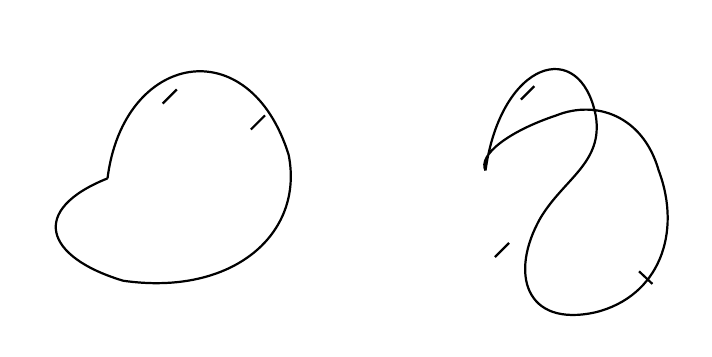
\begin{tikzpicture}[scale=1.0]
\draw[line width=0.8pt] (0,0)
  .. controls (0.2,1.6) and (1.8,1.9) .. (2.3,0.3)
  .. controls (2.5,-0.7) and (1.6,-1.5) .. (0.2,-1.3)
  .. controls (-0.8,-1.0) and (-1.0,-0.4) .. (0,0);
\draw[line width=0.8pt] (0.70,0.95) -- (0.88,1.13);
\draw[line width=0.8pt] (1.82,0.62) -- (2.00,0.80);

\draw[line width=0.8pt] (4.8,0.1)
  .. controls (5.0,1.5) and (6.0,1.8) .. (6.2,0.8)
  .. controls (6.3,0.2) and (5.8,0.0) .. (5.5,-0.5)
  .. controls (5.1,-1.2) and (5.3,-1.9) .. (6.2,-1.7)
  .. controls (7.0,-1.5) and (7.3,-0.7) .. (7.0,0.1)
  .. controls (6.8,0.8) and (6.2,1.0) .. (5.7,0.8)
  .. controls (5.1,0.6) and (4.7,0.3) .. (4.8,0.1);
\draw[line width=0.8pt] (5.25,1.00) -- (5.42,1.17);
\draw[line width=0.8pt] (5.10,-0.82) -- (4.92,-1.00);
\draw[line width=0.8pt] (6.75,-1.18) -- (6.92,-1.34);
\end{tikzpicture}
\caption{Reconstitution nette du cercle et d’une boucle déformée. Une circonférence égale correspond à la même géométrie intrinsèque à une dimension.}
\label{fig:c04-intrinsic-redraw}
\end{figure}

\begin{classroomqa}
\audiencequestion{Un segment de droite fini serait-il le même type d’espace à une dimension ?}
\lecturerresponse{Non. Un segment possède deux extrémités, tandis qu’une boucle fermée n’en a aucune. Cette distinction topologique est intrinsèque et ne peut être supprimée en courbant l’un ou l’autre objet dans un espace plus grand. Une fois la topologie fixée, le segment est caractérisé par sa longueur et la boucle fermée par sa circonférence. \lecturetimestamp{00:26:00--00:26:39}}
\end{classroomqa}

\subsection{Pourquoi les plongements sont utiles, mais facultatifs}

Nous représentons un cercle à une dimension en le plaçant dans un espace à deux dimensions, et une sphère à deux dimensions en la plaçant dans un espace à trois dimensions. Cette démarche nous incite à exiger une quatrième dimension euclidienne avant de parler d’une 3-sphère. Cette exigence tient à notre capacité de visualisation, et non à une nécessité mathématique. Nos capacités visuelles ont évolué pour nous permettre de nous orienter dans un espace à trois dimensions ; les coordonnées et les métriques nous permettent de raisonner au-delà de cette limite sans construire un point de vue extérieur littéral.

\begin{classroomqa}
\audiencequestion{Des dimensions spatiales supplémentaires pourraient-elles exister tout en étant trop petites pour être observées ?}
\lecturerresponse{Oui. La géométrie n’exige pas que toutes les dimensions aient la même étendue observable. Une dimension compacte pourrait être bien plus petite que les échelles accessibles à l’expérience ordinaire. Le point essentiel est toutefois plus simple : que des dimensions supplémentaires existent physiquement ou non, une dimension de plongement n’est pas nécessaire pour définir la métrique intrinsèque de notre espace à trois dimensions. \lecturetimestamp{00:29:55--00:30:12}}
\end{classroomqa}

\begin{classroomqa}
\audiencequestion{Comment un habitant confiné à une ligne courbe pourrait-il savoir si celle-ci est courbée ?}
\lecturerresponse{Il ne le pourrait pas à partir de mesures intrinsèques seules. Imaginons que la lumière et la matière soient confinées dans une fibre optique. Courber la fibre sans l’étirer modifie le plongement, mais pas les distances ni les temps de propagation des signaux mesurés le long de la fibre. Seul un signal qui s’échapperait dans l’espace environnant pourrait révéler la courbure extérieure. \lecturetimestamp{00:30:15--00:31:14}}
\end{classroomqa}

On peut rendre cette expérience de pensée opérationnelle. Une créature confinée à la fibre pourrait émettre un signal, par exemple un photon suffisamment énergétique, et ne découvrir une direction extérieure que si le signal sortait de la fibre puis y revenait en empruntant un trajet impossible selon la métrique à une dimension. De même, l’affirmation selon laquelle l’espace ordinaire possède trois grandes dimensions relève en dernier ressort de l’expérience, et non d’une déduction fondée sur les limites de l’imagination humaine.

\begin{classroomqa}
\audiencequestion{Si tout espace à une dimension est localement plat, tout espace à deux dimensions doit-il aussi être localement plat ?}
\lecturerresponse{Non. Une feuille enroulée en cylindre reste intrinsèquement plate : on peut la dérouler sans l’étirer. On ne peut pas aplatir un hémisphère sur un plan sans l’étirer ni le déchirer ; il possède donc une courbure intrinsèque. Toute petite région suffisamment réduite paraît approximativement euclidienne, mais des écarts mesurables apparaissent à une échelle finie. Le contraste entre un cylindre et une sphère est précisément celui entre courbure extrinsèque et courbure intrinsèque. \lecturetimestamp{00:31:14--00:35:00}}
\end{classroomqa}

\begin{classroomqa}
\audiencequestion{La courbure intrinsèque implique-t-elle nécessairement la présence d’un champ gravitationnel ?}
\lecturerresponse{En relativité générale, la courbure de l’espace-temps est la manifestation invariante de la gravité de marée. La courbure spatiale cosmologique \(k/a^2\) fait donc partie de la géométrie gravitationnelle ; elle ne se réduit pas à une courbure dans un espace extérieur imaginé. La matière influence la courbure par l’équation d’Einstein, mais il ne faut pas en tirer l’affirmation plus forte selon laquelle « la courbure n’existe qu’aux endroits où se trouve la matière » : un espace-temps vide peut porter une courbure de Weyl, comme à l’extérieur d’une étoile ou dans une onde gravitationnelle. \lecturetimestamp{00:35:01--00:35:51}}
\end{classroomqa}

Nous adoptons maintenant l’idéalisation à grande échelle. Faisons une moyenne sur les étoiles, les galaxies, les amas et les irrégularités locales, tout comme on néglige les montagnes lorsqu’on décrit la Terre comme ronde. La géométrie spatiale qui en résulte est supposée homogène et isotrope. Ces hypothèses autorisent trois possibilités à courbure constante : plate, sphérique et hyperbolique.

\section{L’ansatz FRW et les trois cas de courbure}

Les hypothèses de symétrie réduisent la géométrie à un seul facteur dépendant du temps et à un seul signe discret de courbure. En coordonnées comobiles, l’ansatz de Friedmann-Robertson-Walker s’écrit
\begin{equation}
ds^2=-dt^2+a(t)^2\,d\Sigma_k^2,
\qquad
k\in\{-1,0,+1\}.
\label{eq:c04-frw}
\end{equation}
La coordonnée temporelle est le temps propre des observateurs comobiles. L’homogénéité permet à \(a\) de dépendre du temps, mais pas de la position, tandis que l’isotropie interdit toute direction spatiale privilégiée.

\begin{figure}[htbp]
\centering
\includegraphics[width=0.74\textwidth]{lecture_04_figure_02.png}
\caption{Les trois métriques spatiales à courbure constante, regroupées sous le facteur d’échelle commun. Cette image a été capturée plus tard, après que d’autres éléments eurent été ajoutés au tableau, mais elle conserve la discussion sur la métrique de 00:40:23--00:42:42.}
\label{fig:c04-frw-board}
\lectureframe{00:45:48.386}
\end{figure}

Avec une coordonnée radiale \(r\) et la métrique de la sphère unité à deux dimensions \(d\Omega_2^2\), les trois métriques spatiales normalisées sont
\begin{align}
d\Sigma_0^2 &= dr^2+r^2d\Omega_2^2,
&& k=0,
\label{eq:c04-flat-space}\\
d\Sigma_{+1}^2 &= dr^2+\sin^2 r\,d\Omega_2^2,
&& k=+1,
\label{eq:c04-spherical-space}\\
d\Sigma_{-1}^2 &= dr^2+\sinh^2 r\,d\Omega_2^2,
&& k=-1.
\label{eq:c04-hyperbolic-space}
\end{align}
À temps fixé, l’espace est donc plat, à courbure positive ou à courbure négative. Le facteur \(a(t)^2\) modifie toutes les distances spatiales dans la même proportion, tout en préservant la forme normalisée.

Considérons deux galaxies séparées d’une distance comobile \(\Delta\chi\) fixe. Leur distance physique est
\begin{equation}
D(t)=a(t)\Delta\chi.
\end{equation}
En dérivant et en éliminant \(\Delta\chi\), on obtient
\begin{equation}
\dot D=\dot a\,\Delta\chi
      =\frac{\dot a}{a}D
      =H(t)D,
\qquad
H(t)\equiv\frac{\dot a}{a}.
\label{eq:c04-hubble-law}
\end{equation}
La loi de Hubble découle ainsi cinématiquement de la dilatation homogène. Le paramètre de Hubble peut varier dans le temps, mais à chaque instant cosmique donné, il est le même partout.

\section{De l’équation d’Einstein à l’équation de Friedmann}

La métrique nous indique comment mesurer les distances, mais pas comment \(a(t)\) évolue. Un espace-temps courbe exige l’équation d’Einstein. Calculer tous les symboles de Christoffel et toutes les composantes de courbure masquerait l’argument physique ; nous utilisons donc la forme imposée par la symétrie et isolons sa composante temporelle.

Avec \(c=1\) et en omettant provisoirement la constante cosmologique, l’équation tensorielle complète est
\begin{equation}
G_{\mu\nu}
\equiv
R_{\mu\nu}-\frac12 g_{\mu\nu}R
=8\pi G\,T_{\mu\nu}.
\label{eq:c04-einstein}
\end{equation}
Le membre de gauche décrit la géométrie ; celui de droite contient la densité d’énergie, la densité de quantité de mouvement, la pression et les contraintes. Le facteur \(1/3\) ne figure pas dans l’équation tensorielle complète. Il n’apparaît qu’après réduction de la composante temporelle à la forme de Friedmann.

\begin{figure}[htbp]
\centering
\includegraphics[width=0.78\textwidth]{lecture_04_figure_03.png}
\caption{Un état intermédiaire du tableau consacré à l’équation d’Einstein. Le membre géométrique de gauche est visible, mais le tenseur de matière n’est pas encore lisible et la normalisation affichée est incomplète. L’équation~\eqref{eq:c04-einstein} consigne l’équation tensorielle standard, complétée, utilisée dans la dérivation.}
\label{fig:c04-einstein-board}
\lectureframe{00:48:19.394}
\end{figure}

Pour un fluide homogène au repos dans des coordonnées comobiles,
\begin{equation}
T_{00}=\rho.
\label{eq:c04-energy-density}
\end{equation}
Le tenseur d’Einstein temporel possède une propriété structurelle utile. Ses dérivées secondes s’annulent, ne laissant qu’un terme quadratique en dérivée temporelle première et un terme dû à la courbure spatiale :
\begin{equation}
G_{00}=3\left[
\left(\frac{\dot a}{a}\right)^2+\frac{k}{a^2}
\right].
\label{eq:c04-g00}
\end{equation}
En substituant les équations ~\eqref{eq:c04-energy-density} et \eqref{eq:c04-g00} dans l’équation ~\eqref{eq:c04-einstein}, on obtient la première équation de Friedmann,
\begin{equation}
\boxed{
\left(\frac{\dot a}{a}\right)^2+\frac{k}{a^2}
=\frac{8\pi G}{3}\rho
}.
\label{eq:c04-friedmann}
\end{equation}
De manière équivalente,
\begin{equation}
H^2=\frac{8\pi G}{3}\rho-\frac{k}{a^2}.
\label{eq:c04-friedmann-energy}
\end{equation}
L’équation~\eqref{eq:c04-friedmann-energy} a exactement la forme obtenue dans l’argument newtonien précédent. La constante d’intégration y était interprétée comme l’énergie mécanique totale ou la condition d’échappement d’une sphère de matière. En relativité générale, la courbure spatiale intrinsèque occupe le même emplacement mathématique. Cette concordance n’est pas fortuite : dans une région suffisamment petite, les effets de courbure deviennent négligeables et la cosmologie relativiste doit retrouver le comportement newtonien local. La relativité précise aussi que \(\rho\) désigne la densité d’énergie totale ; les particules relativistes et les photons contribuent donc eux aussi à la gravitation, contrairement à ce que laisserait penser un argument fondé sur la seule densité de masse non relativiste.

\begin{classroomqa}
\audiencequestion{Pourquoi la métrique ne comporte-t-elle pas de termes qui mélangent espace et temps ?}
\lecturerresponse{Un terme mixte se comporterait comme un vecteur spatial privilégié ou un écoulement par rapport aux observateurs comobiles. L’homogénéité et l’isotropie exactes ne laissent aucune direction de ce type disponible. Dans des coordonnées adaptées à la matière cosmique, le décalage s’annule donc et la métrique prend la forme par blocs diagonale de l’équation~\eqref{eq:c04-frw}. Si les symétries supposées sont préservées, il ne s’agit pas d’une hypothèse dynamique supplémentaire, mais d’une conséquence géométrique de ces symétries. \lecturetimestamp{00:58:27--00:59:08}}
\end{classroomqa}

\begin{classroomqa}
\audiencequestion{Pourquoi la composante temporelle suffit-elle, et où sont passées les dérivées secondes ?}
\lecturerresponse{L’ansatz homogène et isotrope ne contient qu’une fonction inconnue, \(a(t)\). Les composantes mixtes se réduisent à des identités, tandis que les composantes spatiales sont liées à l’équation temporelle et à la conservation de l’énergie-impulsion. On peut les combiner pour obtenir une équation d’accélération contenant \(\ddot a\), mais le tenseur d’Einstein temporel est particulier : ses termes en dérivées secondes s’annulent, laissant l’équation énergétique du premier ordre~\eqref{eq:c04-friedmann}. Une équation non triviale, accompagnée de la loi d’évolution de la matière, suffit à déterminer l’unique degré de liberté géométrique. \lecturetimestamp{00:59:09--01:00:56}}
\end{classroomqa}

\section{Comment se diluent les constituants de l’Univers}

L’équation de Friedmann n’est pas fermée tant que \(\rho\) n’est pas connue en fonction de \(a\). La géométrie nous a fourni une équation ; la matière présente dans l’Univers doit fournir la seconde relation.

Pour la matière non relativiste, le nombre de particules dans un volume comobile est fixe, tandis que le volume physique croît comme \(a^3\). En négligeant la faible énergie cinétique des particules,
\begin{equation}
\rho_{\mathrm m}(a)=\frac{\rho_{\mathrm m,0}}{a^3}.
\label{eq:c04-matter-scaling}
\end{equation}
La normalisation \(a=1\) peut être fixée à n’importe quelle époque de référence pratique ; seuls les rapports des facteurs d’échelle ont un sens direct.

\begin{classroomqa}
\audiencequestion{Si un univers plat est infini, que signifie le fait que \(a\) tende vers zéro lors du Big Bang ?}
\lecturerresponse{Un espace plat infini reste infini pour toute valeur non nulle de \(a\) ; toutes les distances comobiles finies sont multipliées par le même facteur décroissant. Dans le cas plat, la normalisation absolue de \(a\) est arbitraire ; seul \(a(t_2)/a(t_1)\) a un sens invariant. Pour un univers sphérique fermé, \(a\) correspond naturellement à son rayon de courbure ; dans un univers hyperbolique, il fixe ce rayon. La limite \(a\to0\) signale la singularité cosmologique, et non une boule finie ordinaire placée dans un espace extérieur. \lecturetimestamp{01:05:06--01:05:53}}
\end{classroomqa}

Le rayonnement perd de l’énergie de deux façons. Sa densité numérique diminue comme l’inverse du volume et la longueur d’onde de chaque photon augmente en proportion de \(a\), réduisant son énergie d’un facteur supplémentaire \(a^{-1}\). On a donc
\begin{equation}
\rho_{\mathrm r}(a)=\frac{\rho_{\mathrm r,0}}{a^4}.
\label{eq:c04-radiation-scaling}
\end{equation}
Comme \(a^{-4}\) croît plus vite vers le passé que \(a^{-3}\), le rayonnement domine suffisamment tôt, même si la matière domine bien plus tard.

Si la matière et le rayonnement étaient les seuls constituants, le signe de \(k\) déterminerait fortement le devenir de l’Univers : \(k=+1\) permet un effondrement, \(k=0\) est le cas limite où l’expansion se poursuit éternellement en ralentissant, et \(k=-1\) correspond à une expansion éternelle où la courbure finit par devenir importante. L’énergie noire rompt ce lien simple. Un univers fermé peut se dilater éternellement, et la platitude spatiale ne détermine pas à elle seule le destin ultime de l’Univers.

\section{Équation d’état et loi de continuité}

Plutôt que de mémoriser une loi de dilution différente pour chaque substance, caractérisons la matière par une équation d’état. La démarche comporte deux étapes. Il faut d’abord déduire \(\rho(a)\) à partir d’une relation donnée entre la pression et la densité d’énergie. Il faut ensuite déterminer cette relation à partir de la physique microscopique de la matière, du rayonnement ou du vide. Pour cette leçon, la première étape suffit.

La pression est un flux de quantité de mouvement. Les molécules qui heurtent la paroi d’une boîte inversent leur quantité de mouvement et exercent une poussée sur la paroi ; les particules plus rapides lui transfèrent davantage de quantité de mouvement et produisent une pression plus élevée. Une fois la nature de la matière spécifiée, la densité d’énergie et la pression ne peuvent donc pas être choisies indépendamment. Pour une composante cosmologique simple, on écrit
\begin{equation}
P=w\rho,
\label{eq:c04-equation-state}
\end{equation}
où \(w\) est sans dimension lorsque \(c=1\). La pression de la matière froide est négligeable, donc \(w=0\). Pour le rayonnement, \(w=1/3\) ; le facteur \(1/3\) correspond à la moyenne sur les trois directions spatiales.

\begin{figure}[htbp]
\centering
\includegraphics[width=0.82\textwidth]{lecture_04_figure_06.png}
\caption{Le tableau rassemble les lois d’évolution de la matière et du rayonnement et écrit l’équation d’état sous la forme \(P=W\rho\). Nous utilisons le symbole conventionnel en minuscule \(w\).}
\label{fig:c04-equation-state-board}
\lectureframe{01:15:08.166}
\end{figure}

\subsection{Thermodynamique dans une boîte comobile}

Considérons une boîte comobile de volume physique \(V\), de densité d’énergie \(\rho\) et d’énergie totale
\begin{equation}
E=\rho V.
\end{equation}
Le premier principe s’écrit
\begin{equation}
dE=T\,dS-P\,dV.
\end{equation}
On traite l’expansion cosmologique comme un processus adiabatique, donc \(dS=0\) pour la boîte comobile et
\begin{equation}
dE=-P\,dV.
\label{eq:c04-adiabatic-first-law}
\end{equation}
Le signe moins indique qu’un système en expansion fournit du travail et perd de l’énergie interne. En dérivant séparément \(E=\rho V\), on obtient
\begin{equation}
dE=\rho\,dV+V\,d\rho.
\end{equation}
En égalant les deux expressions,
\begin{align}
\rho\,dV+V\,d\rho&=-P\,dV,\\
V\,d\rho&=-(\rho+P)\,dV.
\label{eq:c04-volume-continuity}
\end{align}
Avec \(P=w\rho\),
\begin{equation}
\frac{d\rho}{\rho}=-(1+w)\frac{dV}{V}.
\end{equation}
L’intégration donne
\begin{equation}
\rho\propto V^{-(1+w)}.
\end{equation}
Puisqu’un volume comobile varie comme \(V\propto a^3\),
\begin{equation}
\boxed{\rho(a)\propto a^{-3(1+w)}}.
\label{eq:c04-density-scaling}
\end{equation}
Sous forme différentielle, la même relation est l’équation locale de conservation de l’énergie :
\begin{equation}
\dot\rho+3H(\rho+P)=0.
\label{eq:c04-continuity}
\end{equation}
Cette loi locale de conservation reste exacte, même si une géométrie cosmologique évolutive n’admet pas nécessairement d’énergie totale conservée à l’échelle globale.

Les deux cas familiers s’obtiennent immédiatement :
\begin{align}
w=0
&\quad\Longrightarrow\quad
\rho_{\mathrm m}\propto a^{-3},\\
w=\frac13
&\quad\Longrightarrow\quad
\rho_{\mathrm r}\propto a^{-4}.
\end{align}
La puissance inverse supplémentaire pour le rayonnement est l’expression thermodynamique du décalage vers le rouge cosmologique.

\begin{classroomqa}
\audiencequestion{Quel rayonnement reste-t-il aujourd’hui dans l’Univers ?}
\lecturerresponse{La discussion en classe porte surtout sur le fond diffus cosmologique, le bain de photons relique de l’Univers chaud primordial. Le rayonnement ne représente aujourd’hui qu’une petite fraction de la densité d’énergie cosmique totale, mais sa loi d’évolution en \(a^{-4}\) signifie qu’il finit par dominer la matière si l’on remonte suffisamment loin dans le temps. Les fractions actuelles précises sont des données observationnelles dont cet argument sur les lois d’évolution n’a pas besoin. \lecturetimestamp{01:26:53--01:28:34}}
\end{classroomqa}

\section{Énergie du vide et échec de la règle liant courbure et destin cosmique}

L’énergie noire introduit l’équation d’état
\begin{equation}
P=-\rho,
\qquad
w=-1.
\label{eq:c04-vacuum-eos}
\end{equation}
Une pression négative correspond à une tension : au lieu de pousser vers l’extérieur sur la paroi d’une boîte, le contenu exerce sur elle une traction vers l’intérieur. Un ressort étiré est un exemple familier de tension, mais il ne s’agit que d’une analogie, et non d’un modèle microscopique de l’énergie du vide.

\begin{classroomqa}
\audiencequestion{La pression négative est-elle liée au zéro absolu ?}
\lecturerresponse{Pas d’une manière générale simple. Refroidir un matériau ordinaire jusqu’à zéro ne produit pas, en soi, l’équation d’état cosmologique \(P=-\rho\). Cet échange est utile, car il distingue la pression thermique de la contrainte du vide : l’énergie du vide se caractérise par un tenseur énergie-impulsion invariant de Lorentz, dont les composantes spatiales agissent comme une pression négative. Son origine microscopique est une question distincte. \lecturetimestamp{01:31:01--01:31:46}}
\end{classroomqa}

En substituant \(w=-1\) dans l’équation~\eqref{eq:c04-density-scaling}, on obtient
\begin{equation}
\rho_\Lambda\propto a^0=\text{constant}.
\label{eq:c04-vacuum-density}
\end{equation}
À mesure qu’une région comobile se dilate, son volume et son énergie totale du vide augmentent ensemble, tandis que l’énergie par unité de volume reste inchangée. Le terme de travail dans l’équation~\eqref{eq:c04-adiabatic-first-law} rend compte de ce comportement, car \(P\) est négative. Dès qu’un tel composant est présent, une courbure spatiale positive ne garantit plus le recollapse.

\begin{classroomqa}
\audiencequestion{Où interviennent la matière noire, les trous noirs et les autres objets compacts ?}
\lecturerresponse{À des échelles grandes par rapport à leurs distances de séparation, tout composant non relativiste dont les vitesses aléatoires sont faibles contribue à la densité de matière sans pression. Cela comprend la matière ordinaire, la matière noire froide et une population d’objets compacts tels que les trous noirs. Leur structure locale est complexe, mais après moyennage à grande échelle, leur équation d’état cosmologique moyenne est approximativement \(w=0\). \lecturetimestamp{01:33:34--01:34:10}}
\end{classroomqa}

\begin{classroomqa}
\audiencequestion{Les équations relativistes reproduisent-elles les solutions dominées par la matière et par le rayonnement obtenues précédemment ?}
\lecturerresponse{Oui. Pour \(k=0\), en substituant \(\rho_{\mathrm m}\propto a^{-3}\) dans l’équation de Friedmann, on obtient \(\dot a^2\propto a^{-1}\) et donc \(a(t)\propto t^{2/3}\). En substituant \(\rho_{\mathrm r}\propto a^{-4}\), on obtient \(\dot a^2\propto a^{-2}\) et \(a(t)\propto t^{1/2}\). La relativité générale en modifie l’interprétation et élargit l’éventail des sources possibles, mais elle préserve ces solutions. \lecturetimestamp{01:34:14--01:35:12}}
\end{classroomqa}

\begin{classroomqa}
\audiencequestion{À quelle force l’énergie noire ressemblerait-elle dans une représentation newtonienne ?}
\lecturerresponse{Une constante cosmologique positive produit une accélération relative répulsive proportionnelle à la séparation :
\[
\ddot D=\frac{\Lambda}{3}D
\]
dans les unités où \(c=1\). Une constante cosmologique négative inverse le signe et produit une attraction. Comme l’effet associé à une valeur positive de \(\Lambda\) croît avec la distance, il peut finir par dominer la matière et la courbure ; même un univers fermé, avec \(k=+1\), peut alors continuer à se dilater. Cette forme newtonienne n’est qu’un reflet utile de la dynamique relativiste. \lecturetimestamp{01:35:13--01:36:55}}
\end{classroomqa}

\section{À retenir}

Le principe cosmologique est une affirmation géométrique portant sur des grandeurs moyennées : après lissage de la structure locale, chaque point et chaque direction sont équivalents. Il restreint la métrique spatiale aux trois cas de courbure constante et rassemble toute la dépendance temporelle dans \(a(t)\) :
\begin{equation}
ds^2=-dt^2+a(t)^2d\Sigma_k^2.
\end{equation}
Les séparations comobiles obéissent alors à \(\dot D=HD\), tandis que les systèmes liés ne sont pas nécessairement entraînés dans ce mouvement.

L’équation temporelle-temporelle d’Einstein transforme l’ansatz en une dynamique :
\begin{equation}
H^2+\frac{k}{a^2}=\frac{8\pi G}{3}\rho.
\end{equation}
Sa ressemblance avec l’équation d’énergie newtonienne est bien réelle, mais la relativité générale identifie le terme jouant le rôle de constante d’intégration à la courbure spatiale intrinsèque et permet à toutes les formes d’énergie de contribuer.

L’apport restant est thermodynamique. Pour un composant en expansion adiabatique tel que \(P=w\rho\),
\begin{equation}
\dot\rho+3H(\rho+P)=0,
\qquad
\rho\propto a^{-3(1+w)}.
\end{equation}
La matière, le rayonnement et l’énergie du vide correspondent respectivement à
\begin{equation}
w=0,\qquad w=\frac13,\qquad w=-1.
\end{equation}
Leurs taux de dilution différents déterminent quel composant gouverne l’expansion à chaque époque. Il s’agit ensuite de comprendre la physique à l’origine de ces équations d’état et de l’accélération produite par l’énergie du vide.
